\documentclass[letterpaper]{article}

\usepackage[utf8]{inputenc}
\usepackage[T1]{fontenc}
\usepackage{textcomp}
\usepackage[dutch]{babel}
\usepackage{amsmath, amssymb}
\usepackage[]{float}
\usepackage[]{braket}
\usepackage[left=50pt, right=50pt]{geometry}% figure support
\usepackage{import}
\usepackage{xifthen}
\pdfminorversion=7
\usepackage{pdfpages}
\usepackage{transparent}
\newcommand{\incfig}[1]{%
	\def\svgwidth{\columnwidth}
	\import{./figures/}{#1.pdf_tex}
}

\pdfsuppresswarningpagegroup=1

\begin{document}

\section*{February 28, 2025}
\hrule 
\

\section*{Majorana Fermion in TFI Model} 


\subsection*{Technical Description}
We start by defining a Hamiltonian 
\begin{equation}
\hat{H} = 
- J \sum_{j} 
\left(
\hat Z_j \hat Z_{j+1} + g \hat X_j
\right)
\end{equation}
where $g$ is a parameter that we are going to tweak. For instance, for $g \to 0 $ 
\[
\hat H  \approx - J \sum_{j} 
\hat Z_j \hat Z_{j+1}
\]
and for $g\to \infty$ 
\[
\hat H  \approx - gJ \sum_{j} 
\hat X_j.
\]
The limit behavior can help us make guesses about the Eigenstates of the Hamiltonian.
\begin{figure}[H]
	\centering
	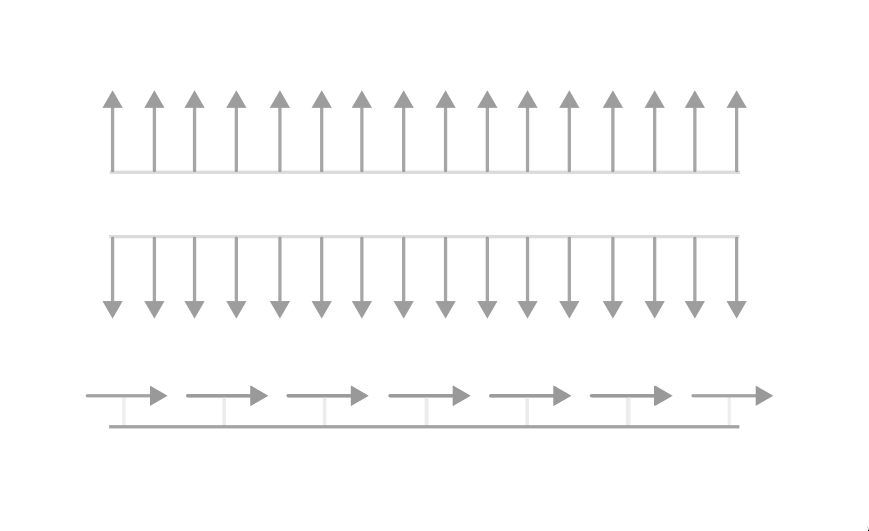
\includegraphics[width=0.8\textwidth]{./figures/nev1.png}
	\caption{Eigenstates for $g\to 0$ and $g\to \infty$}
	\label{fig:-figure-nev1-png}
\end{figure}

Excitations are domain walls. We can define an excitation operator by 
\begin{equation}
	\label{domainwall}
\hat{\tau}_i ^{z} 
\ket{ \uparrow \uparrow \uparrow \cdots}
=
\prod_{j > \overline{i}} \hat{x}_j
\ket{ \uparrow \uparrow \uparrow \cdots}
\end{equation}
where $\overline{i} = i + \frac{1}{2}$. 
\begin{figure}[H]
	\centering
	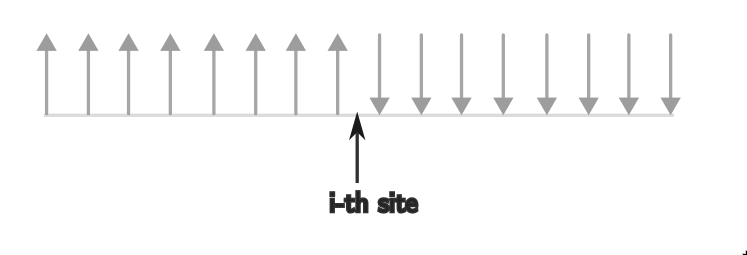
\includegraphics[width=0.8\textwidth]{./figures/nev2.png}
	\caption{Equation \ref{domainwall} visualization.}
	\label{fig:-figures-nev2-png}
\end{figure}

\subsection*{Defining two operators from intuition}

Let's create two definitions inspired by above
\begin{align}
\hat	\chi _j &= \hat{z}_j	\hat{\tau}_{j + \frac{1}{2}}^{z} = 
	z_j \prod_{i > j} x_i  \\ 
\hat{\tilde{\chi}}_j &= \hat{y_j} \hat{\tau}_{j + \frac{1}{2}}^{z} = \underbrace{\hat{y}_j \hat{x}_j}_{- i \hat{z}_j} \hat{x}_j \cdots \hat{x}_j \prod_{i > j} \hat{x}_j = -i z_j \sum_{i \ge j}^{} \hat{x}_i
\end{align}
Intuition for this is: 
\begin{enumerate}
	\item $g\ll 1$, then $\braket{\hat{z}_j } \approx 1$, so $\hat{x}_j \sim \braket{\hat{z}_j } \hat{\tau}_{j + \frac{1}{2}} ^{z} \sim \hat{\tau}_{j+\frac{1}{2}}^{z}$ creates a domain wall. 
	\item $g \gg 1$, then $\hat{\tau}_j ^{z} \approx 1$, so $\hat{x}_j$ and $\hat{\tilde{x}}_j$ flip $\hat{z}_j \to  - \hat{z}_j$. 
\end{enumerate}

\subsection*{Algebra of $\hat{\chi}, \hat{\tilde{\chi}}$ }
For cleanliness we will drop the hats $\hat{\chi} \to  \chi $ for this subsection. 
\begin{align*}
\chi_j ^{T} &= \chi_j \\
\tilde{\chi}_j &= \tilde{\chi} _j\\ 
\underbrace{\chi_i \chi_j}_{\text{WLOG, }i < j} &= z_i \sum_{i' > i }^{} x_i \cdot z_j \sum_{j' > j}^{} x_i = - z_j z_i \cdot \tau_j^{z} \tau_i	^{z} = - \chi_j \chi_i 
\end{align*}

\subsection*{Emergence of Fermions} 
For all $i \neq  j$ here 
\[
	\{ \chi_i, \chi_j \} = 0  \quad  \text{and} \quad 
	\{ \tilde\chi_i, \tilde\chi_j \} = 0  
\]
With the inclusion of the $i = j$ case 
\[
	\{ \chi_i , \chi_j \}  = 2 \delta_{ij} 
\]
This is algebra of Majoranas! 

\subsection*{Jordan-Wigner Transformation} 
\begin{align}
	\hat{c}_j &= \frac{1}{2} \left(\hat{\chi}_j - i \tilde{\hat{\chi}}_j \right)	\\
	\hat{c}_j ^{T}&= \frac{1}{2} \left(\hat{\chi}_j + i \tilde{\hat{\chi}}_j \right)	
\end{align}
There are some helpful properties which are 
\begin{align*}
	\{\hat{c}_i , \hat{c}_j ^{T} \} &= \delta_{ij} \\
	\hat{c}_i ^2 &= 0 
\end{align*}
Let's apply this to the operator $\hat{x}_j$, 
\[
	\hat{x}_j = -i \hat{y}_j \hat{z}_j = - i \hat{y}_j \hat{\tau}_{j + \frac{1}{2}} ^{z} \cdot  
	\hat{z}_j \hat{\tau}_{j+ \frac{1}{2}}^{z} = - i \hat{\tilde{\chi}}_j \hat{\chi}_j
\] 
\[
	\hat{x}_j = 1 - 2 \hat{c}_j ^{T} \hat{c}_j  = (-1)^{\hat{c}_j ^{T} \hat{c}_j}
\]
The last equation above is the Fermion Parity that can be easily shown by the definitions of Jordan-Wigener Transformation. It does the following procedure on a ket
\[
\hat{c}_j ^{T} \hat{c}_j \ket{\rightarrow} _j = 0 
\]
\[
\hat{c}_j ^{T} \hat{c}_j \ket{\leftarrow} _j =  1
\] 
This procedure on a ket can help us count the number of spin flips and domain walls through the following two equations respectively, 
\[
	\text{Number of spin flips } = \text{Number of Fermions } = - \sum_{j}^{} (-1)^{n_j} = +i \sum_{}^{} \hat{\tilde{\chi}}_j \hat{\chi}_j \text{ for } g \gg 1
\]
\[
	\text{Number of Domain Walls }= \sum_{j}^{} \hat{z}_j \hat{z}_{j+1} = 
	\sum_{j}^{} i \hat{\tilde{\chi}} \hat{\chi}_{j+1} \text{ for } g \ll 1 
\]

\subsection*{Re-writing the Hamiltonian} 
We can do the following re-write with the transformation 
\[
	\hat{\mathcal H} _{\text{TFI}} = - J \sum_{j}^{} (\underbrace{i \hat{\tilde{\chi}}_{j+1} \hat\chi_j }_{\text{hopping}} 
	+ \underbrace{g i \hat{\chi}_j \hat{\tilde{\chi}} _j}_{\text{chem. potential}} 
	)
	=
	-J 
	\sum_j \left[\underbrace{
		c_j ^{T} c_{j+1} + c_j ^{T} c_{j+1} ^{T} + \text{h.c.}}_{\text{conserves the number of fermions, i.e. $\mathbb Z_2 $ symmetry}} - 2 g c_j ^{T} c_j	  + g
	\right]
\] 


\subsection*{Dual Fermions} 

\begin{align}
	\gamma_{j+\frac{1}{2}} &= - \tilde{\chi}_{j+1} = i z_{j+1}\cdot  \tau_{j + \frac{3}{2}} ^{z} \\
	\tilde{\gamma}_{j+\frac{1}{2}} &= \chi_j = z_j \cdot  \tau_{j+\frac{1}{2}}^{z} \\
\end{align}

This maps 
\[
	\mathcal H_\text{TFI} = - J \sum_{\overline{j} } 
\left(+ g i \tilde{\gamma}_{\overline{j}+ 1} \gamma_{\overline{j}} + i \tilde{\gamma}_{\overline{j}} \gamma_{\overline{j}}
\right)
\] 

Let's look at the phases now. For $g \ll 1$ we get 
\[
	\mathcal H_{g \to  0 } 
	=
	- J \sum_{\overline{j}}^{} (-1)^{d^{+}_{\overline{j}} d_{\overline{j}} }
	\tag{$d_{\bar{j}} = (1 / 2) (\gamma_{\overline{j}} - i \tilde{\gamma}_{\overline{j}} )$}
\] 
that's where we see new Fermions. The ground state 
\[
	\ket{\text{ground state as } g\to 0} = 
	\ket{\tilde{n}_{\overline{j}} = 0} \to \text{vacuum of fermions by } d_{\overline{j}} 
\]
\[
	d_{\overline{j}} \ket{n_{\overline{j}} = 0} = 0 \tag{for all $j$ } 
\] 
$d^{+}_{\overline{j}} d_{\overline{j}} $ is supposed to count the number of Domain Walls but there are none!

For $g\gg 1$ we get 
\[
	\mathcal H_{g \to  \infty} = - J g \sum_{j} (-1)^{c^{T}_j c_j }
\] 
The ground state
\[
\ket{\text{ground state as } g \to  \infty } = \ket{n_j = 0 } 
\] 
is a vacuum of $c_j$ fermions. Again, $c_j ^{T} c_j$ counts the number of spin flips but there are none!


\subsection*{Relation to Kitaev Chains} 
\[
	\mathcal H_\text{Kitaev} = 
	\sum_j - \frac{(- | \Delta | - + )}{2} i \tilde{\chi}_{j+1} \chi_{j} - 
	\frac{(- | \Delta | + + )}{2} i \chi_j \tilde{\chi}_{j+1} - \frac{i \mu}{2} \tilde{\chi}_j \chi_j 
\] 
Choosing $|\Delta| \to  +$ maps onto the TFI model with $g \to \frac{\mu }{2}$. In particular when $\mu \to  0$ ($g\to 0$), the Kitaev Chain realizes an SPT phase with two unpaired Majorana modes at its ends. This corresponds to $\mathbb Z_2$ topological spin chain in a non-trivial SPT phase. 
\end{document}
